\documentclass[ignorenonframetext,]{beamer}
\setbeamertemplate{caption}[numbered]
\setbeamertemplate{caption label separator}{: }
\setbeamercolor{caption name}{fg=normal text.fg}
\beamertemplatenavigationsymbolsempty
\usepackage{lmodern}
\usepackage{amssymb,amsmath}
\usepackage{ifxetex,ifluatex}
\usepackage{fixltx2e} % provides \textsubscript
\ifnum 0\ifxetex 1\fi\ifluatex 1\fi=0 % if pdftex
  \usepackage[T1]{fontenc}
  \usepackage[utf8]{inputenc}
\else % if luatex or xelatex
  \ifxetex
    \usepackage{mathspec}
  \else
    \usepackage{fontspec}
  \fi
  \defaultfontfeatures{Ligatures=TeX,Scale=MatchLowercase}
    \setmainfont[]{IPAMincho}
\fi
\usefonttheme{serif} % use mainfont rather than sansfont for slide text
% use upquote if available, for straight quotes in verbatim environments
\IfFileExists{upquote.sty}{\usepackage{upquote}}{}
% use microtype if available
\IfFileExists{microtype.sty}{%
\usepackage{microtype}
\UseMicrotypeSet[protrusion]{basicmath} % disable protrusion for tt fonts
}{}
\newif\ifbibliography
\hypersetup{
            pdftitle={Functions - r4ds},
            pdfauthor={Tomoya Fukumoto},
            pdfborder={0 0 0},
            breaklinks=true}
\urlstyle{same}  % don't use monospace font for urls
\usepackage{color}
\usepackage{fancyvrb}
\newcommand{\VerbBar}{|}
\newcommand{\VERB}{\Verb[commandchars=\\\{\}]}
\DefineVerbatimEnvironment{Highlighting}{Verbatim}{commandchars=\\\{\}}
% Add ',fontsize=\small' for more characters per line
\usepackage{framed}
\definecolor{shadecolor}{RGB}{248,248,248}
\newenvironment{Shaded}{\begin{snugshade}}{\end{snugshade}}
\newcommand{\KeywordTok}[1]{\textcolor[rgb]{0.13,0.29,0.53}{\textbf{#1}}}
\newcommand{\DataTypeTok}[1]{\textcolor[rgb]{0.13,0.29,0.53}{#1}}
\newcommand{\DecValTok}[1]{\textcolor[rgb]{0.00,0.00,0.81}{#1}}
\newcommand{\BaseNTok}[1]{\textcolor[rgb]{0.00,0.00,0.81}{#1}}
\newcommand{\FloatTok}[1]{\textcolor[rgb]{0.00,0.00,0.81}{#1}}
\newcommand{\ConstantTok}[1]{\textcolor[rgb]{0.00,0.00,0.00}{#1}}
\newcommand{\CharTok}[1]{\textcolor[rgb]{0.31,0.60,0.02}{#1}}
\newcommand{\SpecialCharTok}[1]{\textcolor[rgb]{0.00,0.00,0.00}{#1}}
\newcommand{\StringTok}[1]{\textcolor[rgb]{0.31,0.60,0.02}{#1}}
\newcommand{\VerbatimStringTok}[1]{\textcolor[rgb]{0.31,0.60,0.02}{#1}}
\newcommand{\SpecialStringTok}[1]{\textcolor[rgb]{0.31,0.60,0.02}{#1}}
\newcommand{\ImportTok}[1]{#1}
\newcommand{\CommentTok}[1]{\textcolor[rgb]{0.56,0.35,0.01}{\textit{#1}}}
\newcommand{\DocumentationTok}[1]{\textcolor[rgb]{0.56,0.35,0.01}{\textbf{\textit{#1}}}}
\newcommand{\AnnotationTok}[1]{\textcolor[rgb]{0.56,0.35,0.01}{\textbf{\textit{#1}}}}
\newcommand{\CommentVarTok}[1]{\textcolor[rgb]{0.56,0.35,0.01}{\textbf{\textit{#1}}}}
\newcommand{\OtherTok}[1]{\textcolor[rgb]{0.56,0.35,0.01}{#1}}
\newcommand{\FunctionTok}[1]{\textcolor[rgb]{0.00,0.00,0.00}{#1}}
\newcommand{\VariableTok}[1]{\textcolor[rgb]{0.00,0.00,0.00}{#1}}
\newcommand{\ControlFlowTok}[1]{\textcolor[rgb]{0.13,0.29,0.53}{\textbf{#1}}}
\newcommand{\OperatorTok}[1]{\textcolor[rgb]{0.81,0.36,0.00}{\textbf{#1}}}
\newcommand{\BuiltInTok}[1]{#1}
\newcommand{\ExtensionTok}[1]{#1}
\newcommand{\PreprocessorTok}[1]{\textcolor[rgb]{0.56,0.35,0.01}{\textit{#1}}}
\newcommand{\AttributeTok}[1]{\textcolor[rgb]{0.77,0.63,0.00}{#1}}
\newcommand{\RegionMarkerTok}[1]{#1}
\newcommand{\InformationTok}[1]{\textcolor[rgb]{0.56,0.35,0.01}{\textbf{\textit{#1}}}}
\newcommand{\WarningTok}[1]{\textcolor[rgb]{0.56,0.35,0.01}{\textbf{\textit{#1}}}}
\newcommand{\AlertTok}[1]{\textcolor[rgb]{0.94,0.16,0.16}{#1}}
\newcommand{\ErrorTok}[1]{\textcolor[rgb]{0.64,0.00,0.00}{\textbf{#1}}}
\newcommand{\NormalTok}[1]{#1}
\usepackage{graphicx,grffile}
\makeatletter
\def\maxwidth{\ifdim\Gin@nat@width>\linewidth\linewidth\else\Gin@nat@width\fi}
\def\maxheight{\ifdim\Gin@nat@height>\textheight0.8\textheight\else\Gin@nat@height\fi}
\makeatother
% Scale images if necessary, so that they will not overflow the page
% margins by default, and it is still possible to overwrite the defaults
% using explicit options in \includegraphics[width, height, ...]{}
\setkeys{Gin}{width=\maxwidth,height=\maxheight,keepaspectratio}

% Prevent slide breaks in the middle of a paragraph:
\widowpenalties 1 10000
\raggedbottom

\AtBeginPart{
  \let\insertpartnumber\relax
  \let\partname\relax
  \frame{\partpage}
}
\AtBeginSection{
  \ifbibliography
  \else
    \let\insertsectionnumber\relax
    \let\sectionname\relax
    \frame{\sectionpage}
  \fi
}
\AtBeginSubsection{
  \let\insertsubsectionnumber\relax
  \let\subsectionname\relax
  \frame{\subsectionpage}
}

\setlength{\parindent}{0pt}
\setlength{\parskip}{6pt plus 2pt minus 1pt}
\setlength{\emergencystretch}{3em}  % prevent overfull lines
\providecommand{\tightlist}{%
  \setlength{\itemsep}{0pt}\setlength{\parskip}{0pt}}
\setcounter{secnumdepth}{0}
\usepackage{zxjatype}
\usepackage[ipa]{zxjafont}

\title{Functions - r4ds}
\author{Tomoya Fukumoto}
\date{2019-07-26}

\begin{document}
\frame{\titlepage}

\begin{frame}{関数}

\begin{block}{神のお言葉}

\begin{quote}
データサイエンティストとしてレベルアップする最高の方法は関数を書くこと
\end{quote}

\end{block}

\begin{block}{関数の利点(コピペに対する)}

\begin{enumerate}
\def\labelenumi{\arabic{enumi}.}
\tightlist
\item
  ある処理の塊に名前を付けて管理できる。

  \begin{itemize}
  \tightlist
  \item
    コードが理解しやすくなる
  \end{itemize}
\item
  変更があったときに一箇所だけ修正すればよい

  \begin{itemize}
  \tightlist
  \item
    生産性UP!
  \end{itemize}
\item
  コピペしたときのミスの可能性を減らせる

  \begin{itemize}
  \tightlist
  \item
    不具合の減少
  \end{itemize}
\end{enumerate}

\end{block}

\end{frame}

\begin{frame}{19.2 When you should you write a function?}

どういうときに関数を書くのか?

A. コピペの回数が2回を上回るとき

{ Don't Repeat Yourself (DRY) principle}

\end{frame}

\begin{frame}[fragile]{関数を書くべき例}

\begin{Shaded}
\begin{Highlighting}[]
\NormalTok{df <-}\StringTok{ }\NormalTok{tibble}\OperatorTok{::}\KeywordTok{tibble}\NormalTok{(}
             \DataTypeTok{a =} \KeywordTok{rnorm}\NormalTok{(}\DecValTok{10}\NormalTok{),}
             \DataTypeTok{b =} \KeywordTok{rnorm}\NormalTok{(}\DecValTok{10}\NormalTok{), }
             \DataTypeTok{c =} \KeywordTok{rnorm}\NormalTok{(}\DecValTok{10}\NormalTok{),}
             \DataTypeTok{d =} \KeywordTok{rnorm}\NormalTok{(}\DecValTok{10}\NormalTok{))}

\NormalTok{df}\OperatorTok{$}\NormalTok{a <-}\StringTok{ }\NormalTok{(df}\OperatorTok{$}\NormalTok{a }\OperatorTok{-}\StringTok{ }\KeywordTok{min}\NormalTok{(df}\OperatorTok{$}\NormalTok{a, }\DataTypeTok{na.rm =} \OtherTok{TRUE}\NormalTok{)) }\OperatorTok{/}
\StringTok{  }\NormalTok{(}\KeywordTok{max}\NormalTok{(df}\OperatorTok{$}\NormalTok{a, }\DataTypeTok{na.rm =} \OtherTok{TRUE}\NormalTok{) }\OperatorTok{-}\StringTok{ }\KeywordTok{min}\NormalTok{(df}\OperatorTok{$}\NormalTok{a, }\DataTypeTok{na.rm =} \OtherTok{TRUE}\NormalTok{))}
\NormalTok{df}\OperatorTok{$}\NormalTok{b <-}\StringTok{ }\NormalTok{(df}\OperatorTok{$}\NormalTok{b }\OperatorTok{-}\StringTok{ }\KeywordTok{min}\NormalTok{(df}\OperatorTok{$}\NormalTok{b, }\DataTypeTok{na.rm =} \OtherTok{TRUE}\NormalTok{)) }\OperatorTok{/}
\StringTok{  }\NormalTok{(}\KeywordTok{max}\NormalTok{(df}\OperatorTok{$}\NormalTok{b, }\DataTypeTok{na.rm =} \OtherTok{TRUE}\NormalTok{) }\OperatorTok{-}\StringTok{ }\KeywordTok{min}\NormalTok{(df}\OperatorTok{$}\NormalTok{a, }\DataTypeTok{na.rm =} \OtherTok{TRUE}\NormalTok{))}
\NormalTok{df}\OperatorTok{$}\NormalTok{c <-}\StringTok{ }\NormalTok{(df}\OperatorTok{$}\NormalTok{c }\OperatorTok{-}\StringTok{ }\KeywordTok{min}\NormalTok{(df}\OperatorTok{$}\NormalTok{c, }\DataTypeTok{na.rm =} \OtherTok{TRUE}\NormalTok{)) }\OperatorTok{/}
\StringTok{  }\NormalTok{(}\KeywordTok{max}\NormalTok{(df}\OperatorTok{$}\NormalTok{c, }\DataTypeTok{na.rm =} \OtherTok{TRUE}\NormalTok{) }\OperatorTok{-}\StringTok{ }\KeywordTok{min}\NormalTok{(df}\OperatorTok{$}\NormalTok{c, }\DataTypeTok{na.rm =} \OtherTok{TRUE}\NormalTok{))}
\NormalTok{df}\OperatorTok{$}\NormalTok{d <-}\StringTok{ }\NormalTok{(df}\OperatorTok{$}\NormalTok{d }\OperatorTok{-}\StringTok{ }\KeywordTok{min}\NormalTok{(df}\OperatorTok{$}\NormalTok{d, }\DataTypeTok{na.rm =} \OtherTok{TRUE}\NormalTok{)) }\OperatorTok{/}
\StringTok{  }\NormalTok{(}\KeywordTok{max}\NormalTok{(df}\OperatorTok{$}\NormalTok{d, }\DataTypeTok{na.rm =} \OtherTok{TRUE}\NormalTok{) }\OperatorTok{-}\StringTok{ }\KeywordTok{min}\NormalTok{(df}\OperatorTok{$}\NormalTok{d, }\DataTypeTok{na.rm =} \OtherTok{TRUE}\NormalTok{))}
\end{Highlighting}
\end{Shaded}

\end{frame}

\begin{frame}[fragile]{関数を書くためのstep1 コードを分析する}

処理の入力は?

\begin{Shaded}
\begin{Highlighting}[]
\NormalTok{(df}\OperatorTok{$}\NormalTok{a }\OperatorTok{-}\StringTok{ }\KeywordTok{min}\NormalTok{(df}\OperatorTok{$}\NormalTok{a, }\DataTypeTok{na.rm =} \OtherTok{TRUE}\NormalTok{)) }\OperatorTok{/}
\StringTok{    }\NormalTok{(}\KeywordTok{max}\NormalTok{(df}\OperatorTok{$}\NormalTok{a, }\DataTypeTok{na.rm =} \OtherTok{TRUE}\NormalTok{) }\OperatorTok{-}\StringTok{ }\KeywordTok{min}\NormalTok{(df}\OperatorTok{$}\NormalTok{a, }\DataTypeTok{na.rm =} \OtherTok{TRUE}\NormalTok{))}
\end{Highlighting}
\end{Shaded}

\begin{block}{答え}

\begin{Shaded}
\begin{Highlighting}[]
\NormalTok{x <-}\StringTok{ }\NormalTok{df}\OperatorTok{$}\NormalTok{a}
\NormalTok{(x }\OperatorTok{-}\StringTok{ }\KeywordTok{min}\NormalTok{(x, }\DataTypeTok{na.rm =} \OtherTok{TRUE}\NormalTok{)) }\OperatorTok{/}
\StringTok{  }\NormalTok{(}\KeywordTok{max}\NormalTok{(x, }\DataTypeTok{na.rm =} \OtherTok{TRUE}\NormalTok{) }\OperatorTok{-}\StringTok{ }\KeywordTok{min}\NormalTok{(x, }\DataTypeTok{na.rm =} \OtherTok{TRUE}\NormalTok{))}
\end{Highlighting}
\end{Shaded}

\end{block}

\end{frame}

\begin{frame}[fragile]{関数を作る}

\begin{Shaded}
\begin{Highlighting}[]
\NormalTok{rescale01 <-}\StringTok{ }\ControlFlowTok{function}\NormalTok{(x) \{}
\NormalTok{  rng <-}\StringTok{ }\KeywordTok{range}\NormalTok{(x, }\DataTypeTok{na.rm =} \OtherTok{TRUE}\NormalTok{)}
\NormalTok{  (x }\OperatorTok{-}\StringTok{ }\NormalTok{rng[}\DecValTok{1}\NormalTok{]) }\OperatorTok{/}\StringTok{ }\NormalTok{(rng[}\DecValTok{2}\NormalTok{] }\OperatorTok{-}\StringTok{ }\NormalTok{rng[}\DecValTok{1}\NormalTok{])}
\NormalTok{\}}
\end{Highlighting}
\end{Shaded}

\begin{block}{方法}

\begin{enumerate}
\def\labelenumi{\arabic{enumi}.}
\tightlist
\item
  関数の名前を決定する

  \begin{itemize}
  \tightlist
  \item
    \texttt{rescale01}
  \end{itemize}
\item
  入力、または引数を\texttt{function}の中に入れる
\item
  関数の内容を\texttt{function(...)}の後に続く\texttt{\{}のブロックで表現
\end{enumerate}

\end{block}

\end{frame}

\begin{frame}[fragile]{関数を使ってコードを書き直す}

\begin{Shaded}
\begin{Highlighting}[]
\NormalTok{df}\OperatorTok{$}\NormalTok{a <-}\StringTok{ }\KeywordTok{rescale01}\NormalTok{(df}\OperatorTok{$}\NormalTok{a)}
\NormalTok{df}\OperatorTok{$}\NormalTok{b <-}\StringTok{ }\KeywordTok{rescale01}\NormalTok{(df}\OperatorTok{$}\NormalTok{b)}
\NormalTok{df}\OperatorTok{$}\NormalTok{c <-}\StringTok{ }\KeywordTok{rescale01}\NormalTok{(df}\OperatorTok{$}\NormalTok{c)}
\NormalTok{df}\OperatorTok{$}\NormalTok{d <-}\StringTok{ }\KeywordTok{rescale01}\NormalTok{(df}\OperatorTok{$}\NormalTok{d)}
\end{Highlighting}
\end{Shaded}

すっきりした!

\begin{block}{まだコピペが残ってるやん}

\(\Rightarrow\) 次の次の章iterationを待て

\end{block}

\end{frame}

\begin{frame}{19.2.1 Practices}

\end{frame}

\begin{frame}{19.3 Functions are for humans and computers}

関数はコンピュータのためだけではなく人間のために書く

\begin{itemize}
\tightlist
\item
  関数名
\item
  コメント
\end{itemize}

\end{frame}

\begin{frame}{関数名の決め方}

\begin{itemize}
\tightlist
\item
  短く、しかし処理の内容を明確に表現したい

  \begin{itemize}
  \tightlist
  \item
    トレードオフになることも多い
  \item
    どちらか一方を選択するとすれば明確にする

    \begin{itemize}
    \tightlist
    \item
      RStudioのオートコンプリート機能
    \end{itemize}
  \end{itemize}
\item
  \textbf{名詞}ではなく\textbf{動詞}で

  \begin{itemize}
  \tightlist
  \item
    引数は名詞
  \item
    動詞が``get''や``compute''ならその目的語(名詞)もあり
  \end{itemize}
\item
  よりよい名前が見つかったら変更することをためらうな
\item
  関数群を作るときは前半部を統一する

  \begin{itemize}
  \tightlist
  \item
    オートコンプリート
  \end{itemize}
\end{itemize}

\end{frame}

\begin{frame}[fragile]{関数名の例}

\begin{Shaded}
\begin{Highlighting}[]
\CommentTok{# Too short}
\KeywordTok{f}\NormalTok{()}

\CommentTok{# Not a verb, or descriptive}
\KeywordTok{my_awesome_function}\NormalTok{()}

\CommentTok{# Long, but clear}
\KeywordTok{impute_missing}\NormalTok{()}
\KeywordTok{collapse_years}\NormalTok{()}
\end{Highlighting}
\end{Shaded}

\end{frame}

\begin{frame}[fragile]{関数群の命名}

\begin{Shaded}
\begin{Highlighting}[]
\CommentTok{# Good}
\KeywordTok{input_select}\NormalTok{()}
\KeywordTok{input_checkbox}\NormalTok{()}
\KeywordTok{input_text}\NormalTok{()}

\CommentTok{# Not so good}
\KeywordTok{select_input}\NormalTok{()}
\KeywordTok{checkbox_input}\NormalTok{()}
\KeywordTok{text_input}\NormalTok{() }
\end{Highlighting}
\end{Shaded}

\end{frame}

\begin{frame}[fragile]{命名規則}

\begin{itemize}
\tightlist
\item
  \texttt{snake\_case}

  \begin{itemize}
  \tightlist
  \item
    Hadleyおすすめ
  \end{itemize}
\item
  \texttt{camelCase}
\end{itemize}

どっちでもいいけど、どちらかに統一するべき

\end{frame}

\begin{frame}[fragile]{コメント}

\texttt{\#}でその行の\texttt{\#}より右側はコメントアウト

\begin{Shaded}
\begin{Highlighting}[]
\CommentTok{# this is comment}
\NormalTok{a <-}\StringTok{ }\NormalTok{pi }\CommentTok{#this also comment}
\end{Highlighting}
\end{Shaded}

\begin{itemize}
\tightlist
\item
  コメントは「なぜ」その処理をするのかを書くべし

  \begin{itemize}
  \tightlist
  \item
    「何を」「どのようにして」では\textbf{無い}
  \end{itemize}
\item
  なぜ

  \begin{itemize}
  \tightlist
  \item
    中間変数を置いたのか?
  \item
    2つの関数に分けたのか?
  \item
    他の方法は試したけどうまくいかなかったのか?
  \end{itemize}
\item
  なぜこのようなコードになったのか?
\end{itemize}

\end{frame}

\begin{frame}{コメントを書かないと}

\begin{figure}
\centering
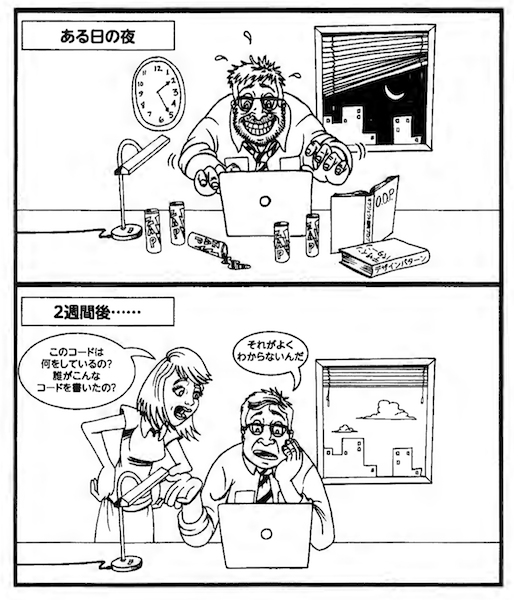
\includegraphics{../img/2018-1-2-9-readable-code.png}
\caption{Readable Code}
\end{figure}

\end{frame}

\begin{frame}[fragile]{コードセクション(Rstudio)}

次のコードを使えばRStdudioでセクション区切りとみなされる

\begin{Shaded}
\begin{Highlighting}[]
\CommentTok{# Load data --------------------------------------}

\CommentTok{# Plot data --------------------------------------}
\end{Highlighting}
\end{Shaded}

\begin{figure}
\centering
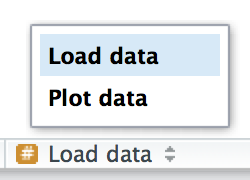
\includegraphics[width=0.72917in]{../img/rstudio-nav.png}
\caption{Tstudio}
\end{figure}

\begin{block}{キーボード・ショートカット}

Ctrl + Shift + R

\end{block}

\end{frame}

\begin{frame}{19.3.1 Exercises}

\end{frame}

\begin{frame}[fragile]{19.4 Condition execution}

\texttt{if}関数を使った条件分岐

\begin{Shaded}
\begin{Highlighting}[]
\ControlFlowTok{if}\NormalTok{ (condition) \{}
    \CommentTok{# code executed when condition is TRUE}
\NormalTok{\} }\ControlFlowTok{else}\NormalTok{ \{}
    \CommentTok{# code executed when condition is FALSE}
\NormalTok{\}}
\end{Highlighting}
\end{Shaded}

\end{frame}

\begin{frame}[fragile]{19.4.1 Conditions}

\begin{Shaded}
\begin{Highlighting}[]
\ControlFlowTok{if}\NormalTok{ (condition) \{}
    \CommentTok{# code executed when condition is TRUE}
\NormalTok{\} }\ControlFlowTok{else}\NormalTok{ \{}
    \CommentTok{# code executed when condition is FALSE}
\NormalTok{\}}
\end{Highlighting}
\end{Shaded}

conditionは\texttt{TRUE}か\texttt{FALSE}かのどちらか

\begin{itemize}
\tightlist
\item
  ベクトルは基本NO!

  \begin{itemize}
  \tightlist
  \item
    入るとwarningを出して一番先頭の値だけ採用
  \item
    でも使うのは推奨しません
  \end{itemize}
\item
  \texttt{NA}はエラー
\end{itemize}

\end{frame}

\begin{frame}[fragile]{Condition内での演算}

\begin{block}{\texttt{\&\&}や\texttt{\textbar{}\textbar{}}はANDやORの役割}

実際の働きは前から順に評価して\texttt{TRUE}や\texttt{FALSE}が出たら打ち切り
- 後ろにエラーがあっても問題なく走る

\end{block}

\begin{block}{ベクトル化関数に注意}

\begin{itemize}
\tightlist
\item
  \texttt{\&}や\texttt{\textbar{}}は使うな

  \begin{itemize}
  \tightlist
  \item
    関数\texttt{any}, \texttt{all}
  \end{itemize}
\item
  \texttt{==}も使うな

  \begin{itemize}
  \tightlist
  \item
    関数\texttt{identical}, \texttt{near}
  \end{itemize}
\end{itemize}

\end{block}

\end{frame}

\begin{frame}[fragile]{19.4.2 Multiple Contitions}

\begin{Shaded}
\begin{Highlighting}[]
\ControlFlowTok{if}\NormalTok{ (this) \{}
    \CommentTok{# do that}
\NormalTok{\} }\ControlFlowTok{else} \ControlFlowTok{if}\NormalTok{ (that) \{}
    \CommentTok{# do something else}
\NormalTok{\} }\ControlFlowTok{else}\NormalTok{ \{}
    \CommentTok{# }
\NormalTok{\}}
\end{Highlighting}
\end{Shaded}

\end{frame}

\begin{frame}[fragile]{19.4.3 Code style}

インデントと改行の作法

\begin{itemize}
\tightlist
\item
  \texttt{\{}と\texttt{\}}の間の行はインデントを入れる

  \begin{itemize}
  \tightlist
  \item
    半角スペース2個がおすすめ
  \end{itemize}
\item
  \texttt{\{}の直前は改行しない。直後は改行
\item
  \texttt{\}}の直前に改行し、直後は\texttt{else}の場合を除いて改行
\end{itemize}

\end{frame}

\begin{frame}{19.4.4 Exercises}

\end{frame}

\begin{frame}{19.5 Function arguments}

関数の引数

\end{frame}

\begin{frame}[fragile]{データと詳細}

関数の引数は\textbf{data}と\textbf{details}の二種に分類できる

\begin{itemize}
\tightlist
\item
  関数\texttt{log}は\texttt{x}がdataで\texttt{base}がdetail
\item
  関数\texttt{mean}は\texttt{x}がdataで\texttt{trim},\texttt{na.rm}がdetails
\item
  関数\texttt{t.test}は\texttt{x},\texttt{y}がdataで、\texttt{alternative},\texttt{mu},\texttt{paired},\texttt{var.equal},\texttt{conf.level}がdetials
\item
  関数\texttt{str\_c}は\texttt{...}がdata,
  \texttt{sep},\texttt{collapse}がdetails
\end{itemize}

普通はdataが先で、detailsにはデフォルト値が存在

\end{frame}

\begin{frame}[fragile]{デフォルト値}

\begin{Shaded}
\begin{Highlighting}[]
\NormalTok{mean_ci <-}\StringTok{ }\ControlFlowTok{function}\NormalTok{(x, }\DataTypeTok{conf =} \FloatTok{0.95}\NormalTok{) \{}
\NormalTok{    se <-}\StringTok{ }\KeywordTok{sd}\NormalTok{(x) }\OperatorTok{/}\StringTok{ }\KeywordTok{sqrt}\NormalTok{(}\KeywordTok{length}\NormalTok{(x))}
\NormalTok{  alpha <-}\StringTok{ }\DecValTok{1} \OperatorTok{-}\StringTok{ }\NormalTok{conf}
    \KeywordTok{mean}\NormalTok{(x) }\OperatorTok{+}\StringTok{ }\NormalTok{se }\OperatorTok{*}\StringTok{ }\KeywordTok{qnorm}\NormalTok{(}\KeywordTok{c}\NormalTok{(alpha }\OperatorTok{/}\StringTok{ }\DecValTok{2}\NormalTok{, }\DecValTok{1} \OperatorTok{-}\StringTok{ }\NormalTok{alpha }\OperatorTok{/}\StringTok{ }\DecValTok{2}\NormalTok{))}
\NormalTok{\}}
\end{Highlighting}
\end{Shaded}

\begin{itemize}
\tightlist
\item
  一般的な値か安全サイドの値

  \begin{itemize}
  \tightlist
  \item
    \texttt{na.rm=FALSE}
  \end{itemize}
\end{itemize}

\end{frame}

\begin{frame}[fragile]{引数名の指定方法}

\begin{Shaded}
\begin{Highlighting}[]
\CommentTok{# Good}
\KeywordTok{mean}\NormalTok{(}\DecValTok{1}\OperatorTok{:}\DecValTok{10}\NormalTok{, }\DataTypeTok{na.rm =} \OtherTok{TRUE}\NormalTok{)}
\KeywordTok{mean}\NormalTok{(}\DataTypeTok{na.rm =} \OtherTok{TRUE}\NormalTok{, }\DecValTok{1}\OperatorTok{:}\DecValTok{10}\NormalTok{)}

\CommentTok{# Bad}
\KeywordTok{mean}\NormalTok{(}\DataTypeTok{x =} \DecValTok{1}\OperatorTok{:}\DecValTok{10}\NormalTok{, , }\OtherTok{FALSE}\NormalTok{)}
\KeywordTok{mean}\NormalTok{(, }\OtherTok{TRUE}\NormalTok{, }\DataTypeTok{x =} \KeywordTok{c}\NormalTok{(}\DecValTok{1}\OperatorTok{:}\DecValTok{10}\NormalTok{, }\OtherTok{NA}\NormalTok{))}
\end{Highlighting}
\end{Shaded}

\begin{itemize}
\tightlist
\item
  関数をコールするとき引数名は省略可能

  \begin{itemize}
  \tightlist
  \item
    前から順番に割り当てられる
  \end{itemize}
\item
  名前を指定すれば順番はめちゃくちゃでもいい
\end{itemize}

\end{frame}

\begin{frame}[fragile]{Coding style}

\begin{itemize}
\tightlist
\item
  引数名を指定する\texttt{=}の前後にはスペース入れろ
\item
  引数値の後ろの\texttt{,}の直前はスペース無し、直後はスペースあり
\end{itemize}

\begin{Shaded}
\begin{Highlighting}[]
\KeywordTok{mean}\NormalTok{(}\DecValTok{1}\OperatorTok{:}\DecValTok{10}\NormalTok{, }\DataTypeTok{na.rm =} \OtherTok{TRUE}\NormalTok{)}
\end{Highlighting}
\end{Shaded}

\end{frame}

\begin{frame}[fragile]{19.5.1 Choosing names}

一般的な引数名の割当

\begin{itemize}
\tightlist
\item
  \texttt{x},\texttt{y},\texttt{z}はベクトル
\item
  \texttt{w}はベクトルの重み
\item
  \texttt{df}はデータフレーム
\item
  \texttt{i},\texttt{j}は整数インデックス
\item
  \texttt{n}は長さや行数(自然数)
\item
  \texttt{p}は列数
\end{itemize}

固執する必要は無いが参考にはなる

\end{frame}

\begin{frame}[fragile]{19.5.2 Checking values}

引数の値が正確かチェック

\begin{Shaded}
\begin{Highlighting}[]
\NormalTok{wt_mean <-}\StringTok{ }\ControlFlowTok{function}\NormalTok{(x, w) \{}
    \ControlFlowTok{if}\NormalTok{ (}\KeywordTok{length}\NormalTok{(x) }\OperatorTok{!=}\StringTok{ }\KeywordTok{length}\NormalTok{(w)) \{}
          \KeywordTok{stop}\NormalTok{(}\StringTok{"`x` and `w` must be the same length"}\NormalTok{, }\DataTypeTok{call. =} \OtherTok{FALSE}\NormalTok{)}
\NormalTok{  \}}
  \KeywordTok{sum}\NormalTok{(w }\OperatorTok{*}\StringTok{ }\NormalTok{x) }\OperatorTok{/}\StringTok{ }\KeywordTok{sum}\NormalTok{(w)}
\NormalTok{\}}
\end{Highlighting}
\end{Shaded}

\end{frame}

\begin{frame}[fragile]{限度ってもんがある}

\begin{Shaded}
\begin{Highlighting}[]
\NormalTok{wt_mean <-}\StringTok{ }\ControlFlowTok{function}\NormalTok{(x, w, }\DataTypeTok{na.rm =} \OtherTok{FALSE}\NormalTok{) \{}
  \ControlFlowTok{if}\NormalTok{ (}\OperatorTok{!}\KeywordTok{is.logical}\NormalTok{(na.rm)) \{}
    \KeywordTok{stop}\NormalTok{(}\StringTok{"`na.rm` must be logical"}\NormalTok{)}
\NormalTok{  \}}
  \ControlFlowTok{if}\NormalTok{ (}\KeywordTok{length}\NormalTok{(na.rm) }\OperatorTok{!=}\StringTok{ }\DecValTok{1}\NormalTok{) \{}
    \KeywordTok{stop}\NormalTok{(}\StringTok{"`na.rm` must be length 1"}\NormalTok{)}
\NormalTok{  \}}
  \ControlFlowTok{if}\NormalTok{ (}\KeywordTok{length}\NormalTok{(x) }\OperatorTok{!=}\StringTok{ }\KeywordTok{length}\NormalTok{(w)) \{}
    \KeywordTok{stop}\NormalTok{(}\StringTok{"`x` and `w` must be the same length"}\NormalTok{, }\DataTypeTok{call. =} \OtherTok{FALSE}\NormalTok{)}
\NormalTok{  \} }
  \ControlFlowTok{if}\NormalTok{ (na.rm) \{}
\NormalTok{    miss <-}\StringTok{ }\KeywordTok{is.na}\NormalTok{(x) }\OperatorTok{|}\StringTok{ }\KeywordTok{is.na}\NormalTok{(w)}
\NormalTok{    x <-}\StringTok{ }\NormalTok{x[}\OperatorTok{!}\NormalTok{miss]}
\NormalTok{    w <-}\StringTok{ }\NormalTok{w[}\OperatorTok{!}\NormalTok{miss]}
\NormalTok{  \}}
  \KeywordTok{sum}\NormalTok{(w }\OperatorTok{*}\StringTok{ }\NormalTok{x) }\OperatorTok{/}\StringTok{ }\KeywordTok{sum}\NormalTok{(w)}
\NormalTok{\}}
\end{Highlighting}
\end{Shaded}

\end{frame}

\begin{frame}[fragile]{\texttt{stopifnot}}

\begin{Shaded}
\begin{Highlighting}[]
\NormalTok{wt_mean <-}\StringTok{ }\ControlFlowTok{function}\NormalTok{(x, w, }\DataTypeTok{na.rm =} \OtherTok{FALSE}\NormalTok{) \{}
  \KeywordTok{stopifnot}\NormalTok{(}\KeywordTok{is.logical}\NormalTok{(na.rm), }\KeywordTok{length}\NormalTok{(na.rm) }\OperatorTok{==}\StringTok{ }\DecValTok{1}\NormalTok{)}
  \KeywordTok{stopifnot}\NormalTok{(}\KeywordTok{length}\NormalTok{(x) }\OperatorTok{==}\StringTok{ }\KeywordTok{length}\NormalTok{(w)) }
  \ControlFlowTok{if}\NormalTok{ (na.rm) \{}
\NormalTok{    miss <-}\StringTok{ }\KeywordTok{is.na}\NormalTok{(x) }\OperatorTok{|}\StringTok{ }\KeywordTok{is.na}\NormalTok{(w)}
\NormalTok{    x <-}\StringTok{ }\NormalTok{x[}\OperatorTok{!}\NormalTok{miss]}
\NormalTok{    w <-}\StringTok{ }\NormalTok{w[}\OperatorTok{!}\NormalTok{miss]}
\NormalTok{  \}}
  \KeywordTok{sum}\NormalTok{(w }\OperatorTok{*}\StringTok{ }\NormalTok{x) }\OperatorTok{/}\StringTok{ }\KeywordTok{sum}\NormalTok{(w)}
\NormalTok{\}}
\end{Highlighting}
\end{Shaded}

\begin{itemize}
\tightlist
\item
  エラー条件ではなく、有るべき条件を指定できる
\end{itemize}

\end{frame}

\begin{frame}[fragile]{19.5.3 Dot-dot-dot (\ldots{})}

任意の数の引数を受ける関数

\begin{block}{例}

\begin{Shaded}
\begin{Highlighting}[]
\KeywordTok{sum}\NormalTok{(}\DecValTok{1}\NormalTok{, }\DecValTok{2}\NormalTok{, }\DecValTok{3}\NormalTok{, }\DecValTok{4}\NormalTok{, }\DecValTok{5}\NormalTok{, }\DecValTok{6}\NormalTok{, }\DecValTok{7}\NormalTok{, }\DecValTok{8}\NormalTok{, }\DecValTok{9}\NormalTok{, }\DecValTok{10}\NormalTok{)}
\CommentTok{#> [1] 55}
\NormalTok{stringr}\OperatorTok{::}\KeywordTok{str_c}\NormalTok{(}\StringTok{"a"}\NormalTok{, }\StringTok{"b"}\NormalTok{, }\StringTok{"c"}\NormalTok{, }\StringTok{"d"}\NormalTok{, }\StringTok{"e"}\NormalTok{, }\StringTok{"f"}\NormalTok{)}
\CommentTok{#> [1] "abcdef"}
\end{Highlighting}
\end{Shaded}

\end{block}

\end{frame}

\begin{frame}[fragile]{\texttt{...}}

\begin{Shaded}
\begin{Highlighting}[]
\NormalTok{rule <-}\StringTok{ }\ControlFlowTok{function}\NormalTok{(..., }\DataTypeTok{pad =} \StringTok{"-"}\NormalTok{) \{}
\NormalTok{  title <-}\StringTok{ }\KeywordTok{paste0}\NormalTok{(...)}
\NormalTok{  width <-}\StringTok{ }\KeywordTok{getOption}\NormalTok{(}\StringTok{"width"}\NormalTok{) }\OperatorTok{-}\StringTok{ }\KeywordTok{nchar}\NormalTok{(title) }\OperatorTok{-}\StringTok{ }\DecValTok{5}
  \KeywordTok{cat}\NormalTok{(title, }\StringTok{" "}\NormalTok{, stringr}\OperatorTok{::}\KeywordTok{str_dup}\NormalTok{(pad, width), }\StringTok{"}\CharTok{\textbackslash{}n}\StringTok{"}\NormalTok{, }\DataTypeTok{sep =} \StringTok{""}\NormalTok{)}
\NormalTok{\}}
\KeywordTok{rule}\NormalTok{(}\StringTok{"Important output"}\NormalTok{) }
\end{Highlighting}
\end{Shaded}

\begin{verbatim}
## Important output ------------------------------------------------------
\end{verbatim}

関数がコールされたときに指定された引数で引数名が割当られなかったら\texttt{...}に入る

\end{frame}

\begin{frame}[fragile]{19.4.5 Lazy evaluation}

遅延評価。引数の値は実際に必要とされるまでは評価されない

\begin{Shaded}
\begin{Highlighting}[]
\NormalTok{x <-}\StringTok{ }\OtherTok{FALSE}
\NormalTok{f <-}\StringTok{ }\ControlFlowTok{function}\NormalTok{(}\DataTypeTok{y =}\NormalTok{ x <-}\StringTok{ }\OtherTok{TRUE}\NormalTok{, z)\{}
  \ControlFlowTok{if}\NormalTok{(z)\{}
    \KeywordTok{return}\NormalTok{(x)}
\NormalTok{  \}}\ControlFlowTok{else} \ControlFlowTok{if}\NormalTok{(y)\{}
    \KeywordTok{return}\NormalTok{(x)}
\NormalTok{  \}}
\NormalTok{\}}
\KeywordTok{f}\NormalTok{(}\DataTypeTok{z =} \OtherTok{TRUE}\NormalTok{)}
\end{Highlighting}
\end{Shaded}

\begin{verbatim}
## [1] FALSE
\end{verbatim}

\begin{Shaded}
\begin{Highlighting}[]
\KeywordTok{f}\NormalTok{(}\DataTypeTok{z =} \OtherTok{FALSE}\NormalTok{)}
\end{Highlighting}
\end{Shaded}

\begin{verbatim}
## [1] TRUE
\end{verbatim}

\end{frame}

\begin{frame}{19.5.5 Exercises}

\end{frame}

\begin{frame}{19.6 Return values}

戻り値

関数をコールした結果得られるオブジェクト

\end{frame}

\begin{frame}[fragile]{19.6.1 Explicit return statement}

デフォルトは関数内で最後に実行されたオブジェクトが戻り値になる

関数\texttt{return}を使って、明示的にリターンを設定することでコードを読みやすくできる

\begin{Shaded}
\begin{Highlighting}[]
\NormalTok{complicated_function <-}\StringTok{ }\ControlFlowTok{function}\NormalTok{(x, y, z) \{}
  \ControlFlowTok{if}\NormalTok{ (}\KeywordTok{length}\NormalTok{(x) }\OperatorTok{==}\StringTok{ }\DecValTok{0} \OperatorTok{||}\StringTok{ }\KeywordTok{length}\NormalTok{(y) }\OperatorTok{==}\StringTok{ }\DecValTok{0}\NormalTok{) \{}
    \KeywordTok{return}\NormalTok{(}\DecValTok{0}\NormalTok{)}
\NormalTok{  \} }
  \CommentTok{# Complicated code here}
\NormalTok{\}}
\end{Highlighting}
\end{Shaded}

\end{frame}

\begin{frame}{19.6.2 Writing pipeable functions}

自作関数をパイプラインに繋げる

\end{frame}

\begin{frame}[fragile]{二種類のパイプライン接続関数}

\begin{itemize}
\tightlist
\item
  変換

  \begin{itemize}
  \tightlist
  \item
    関数の入力データと戻り値とが同一のデータ型だとつないでいける
  \end{itemize}
\item
  副作用

  \begin{itemize}
  \tightlist
  \item
    プロットしたり文字列を表示したり
  \item
    戻り値は入力データそのもの。しかしinvisibleであるべき
  \end{itemize}
\end{itemize}

\begin{block}{副作用の例}

\begin{Shaded}
\begin{Highlighting}[]
\NormalTok{show_missings <-}\StringTok{ }\ControlFlowTok{function}\NormalTok{(df) \{}
\NormalTok{  n <-}\StringTok{ }\KeywordTok{sum}\NormalTok{(}\KeywordTok{is.na}\NormalTok{(df))}
  \KeywordTok{cat}\NormalTok{(}\StringTok{"Missing values: "}\NormalTok{, n, }\StringTok{"}\CharTok{\textbackslash{}n}\StringTok{"}\NormalTok{, }\DataTypeTok{sep =} \StringTok{""}\NormalTok{) }
  \KeywordTok{invisible}\NormalTok{(df)}
\NormalTok{\}}
\end{Highlighting}
\end{Shaded}

\end{block}

\end{frame}

\begin{frame}{19.7 Environment}

Rでの関数の扱い

\end{frame}

\begin{frame}[fragile]{レキシカルスコープ}

\begin{Shaded}
\begin{Highlighting}[]
\NormalTok{f <-}\StringTok{ }\ControlFlowTok{function}\NormalTok{(x) \{}
\NormalTok{  x }\OperatorTok{+}\StringTok{ }\NormalTok{y}
\NormalTok{\} }
\NormalTok{y <-}\StringTok{ }\DecValTok{100}
\KeywordTok{f}\NormalTok{(}\DecValTok{10}\NormalTok{) }
\end{Highlighting}
\end{Shaded}

\begin{verbatim}
## [1] 110
\end{verbatim}

\begin{Shaded}
\begin{Highlighting}[]
\NormalTok{y <-}\StringTok{ }\DecValTok{1000}
\KeywordTok{f}\NormalTok{(}\DecValTok{10}\NormalTok{)}
\end{Highlighting}
\end{Shaded}

\begin{verbatim}
## [1] 1010
\end{verbatim}

\end{frame}

\begin{frame}{参考文献}

\begin{itemize}
\tightlist
\item
  \url{https://rion778.hatenablog.com/entry/2015/05/31/175055}
\item
  \url{http://adv-r.had.co.nz/Functions.html\#lazy-evaluation}
\end{itemize}

\end{frame}

\end{document}
